\begin{answer}
\begin{figure}[H]
  \centering

  \begin{subfigure}[b]{0.48\textwidth}
    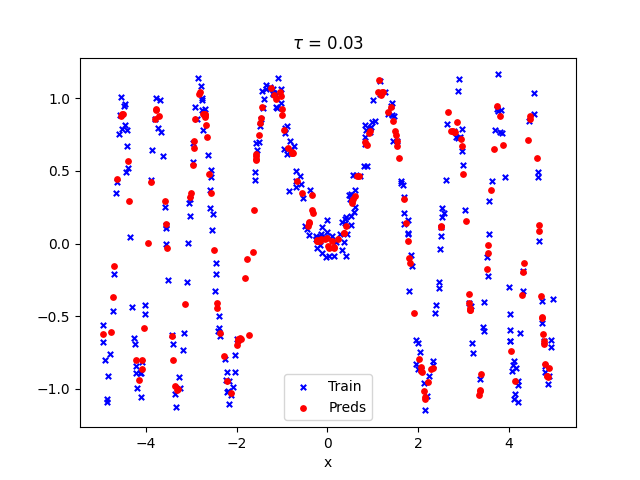
\includegraphics[width=\textwidth]{lwr/tau=0.03.png}
    \caption*{\(\tau = 0.03\)}
  \end{subfigure}
  \hfill
  \begin{subfigure}[b]{0.48\textwidth}
    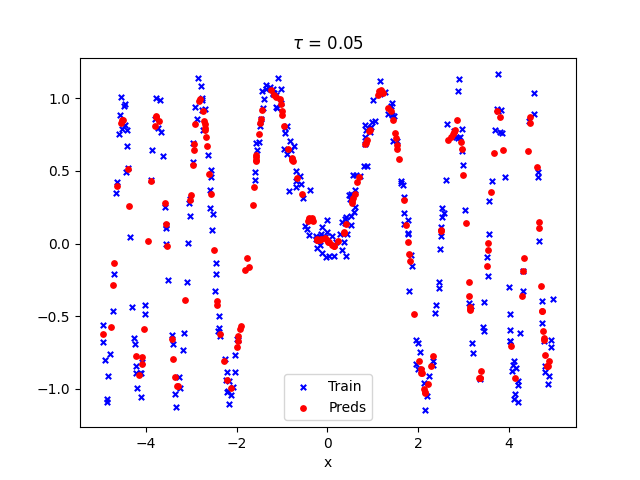
\includegraphics[width=\textwidth]{lwr/tau=0.05.png}
    \caption*{\(\tau = 0.05\)}
  \end{subfigure}

  \vspace{0.02\textheight} % Adjust the vertical space between rows

  \begin{subfigure}[b]{0.48\textwidth}
    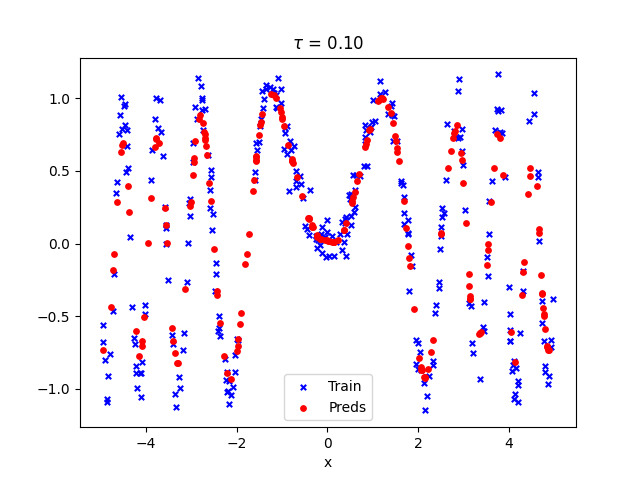
\includegraphics[width=\textwidth]{lwr/tau=0.1.png}
    \caption*{\(\tau = 0.1\)}
  \end{subfigure}
  \hfill
  \begin{subfigure}[b]{0.48\textwidth}
    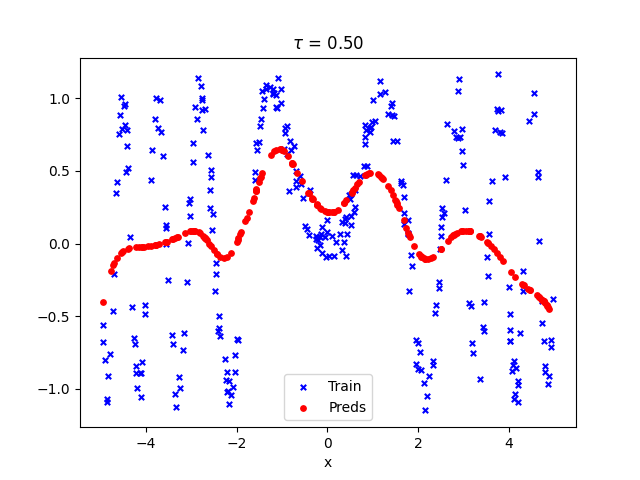
\includegraphics[width=\textwidth]{lwr/tau=0.5.png}
    \caption*{\(\tau = 0.5\)}
  \end{subfigure}

  \vspace{0.02\textheight} % Adjust the vertical space between rows

  \begin{subfigure}[b]{0.48\textwidth}
    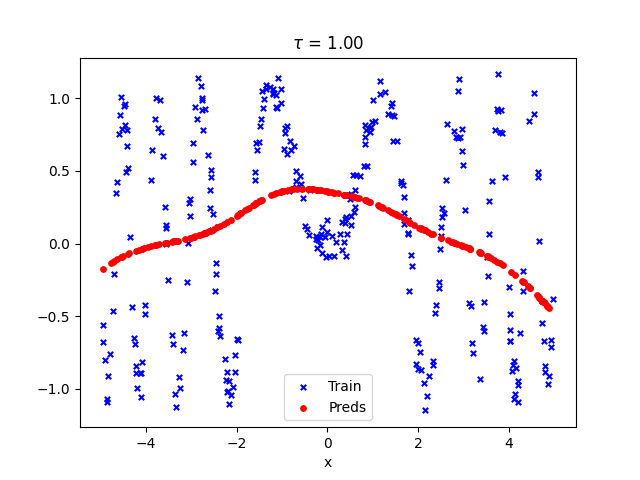
\includegraphics[width=\textwidth]{lwr/tau=1.0.png}
    \caption*{\(\tau = 1\)}
  \end{subfigure}
  \hfill
  \begin{subfigure}[b]{0.48\textwidth}
    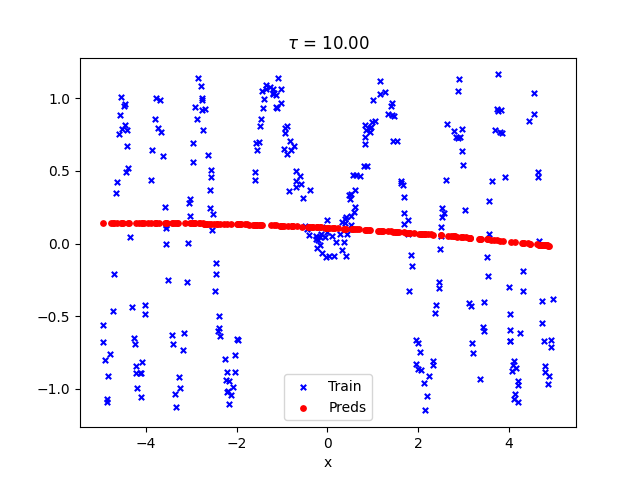
\includegraphics[width=\textwidth]{lwr/tau=10.0.png}
    \caption*{\(\tau = 10\)}
  \end{subfigure}
\end{figure}

The optimal $\tau$ is $\tau = 0.05$ that got $MSE$ 0.0124 on the validation set, the $MSE$ on the test set for that value is 0.0169.

\end{answer}
